\section{Exploration de termes sous forme de graphe RDF}

Afin de visualiser les résultats de Word2Vec formatés en RDF, nous avons créé une première ontologie modélisée sur Word2Vec. Elle sert de premier palier en vue du peuplement d'ontologies métiers.
%
\begin{figure}[tb]
    \begin{center}
        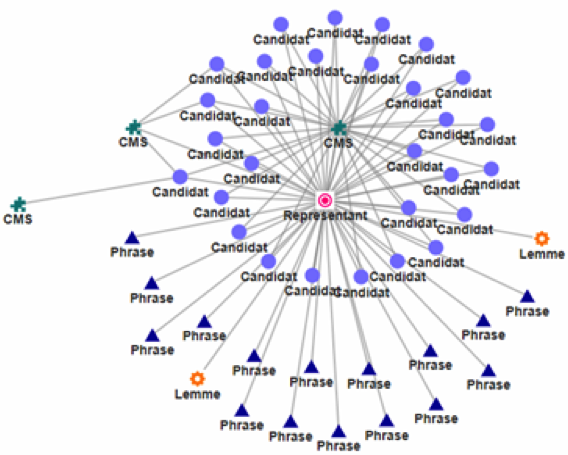
\includegraphics[width=7cm]{figures/gtype}
    \end{center}
    \caption{Modélisation des résultats Word2Vec}\label{fig:gtype}
\end{figure}
%
Nous produisons une visualisation sous forme de graphe où pour chaque mot du corpus, considéré comme étant de type \texttt{Representant}, nous affichons ses quinze termes candidats (classe \texttt{Candidat}) les plus similaires.
Pour visualiser ces résultats, nous avons utilisé l'outil SemVue développé à EDF. Cet outil propose une interface de navigation dans un graphe RDF extrêmement facile à mettre en œuvre à chaque étape du développement d’un entrepôt de données. Le cœur de l’interface est défini à l’aide d’une ontologie associée à la modélisation métier proprement dite dans un entrepôt de données \cite{mnpho14parallel-materialisation-RDFox} et permet ainsi à l’interface web de lancer des requêtes SPARQL. La stratégie d’affichage de SemVue est définie à l’aide d’axiomes OWL, ceux-ci configurant dynamiquement le sous-graphe à exposer à l’utilisateur.
Grâce à cette visualisation nous avons d'optimisé de manière itérative le paramétrage de Word2Vec et validé qualitativement nos résultats (fig \ref{fig:w2v}).
%
\begin{figure}[tb]
    \begin{center}
        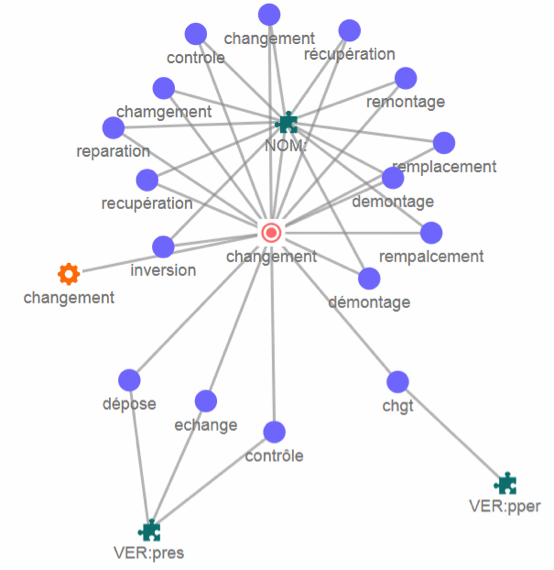
\includegraphics[width=7cm]{figures/w2v}
    \end{center}
    \caption{Graphe sur le mot "changement"}\label{fig:w2v}
\end{figure}
%
